\documentclass{article}
\usepackage{xeCJK,amsmath,geometry,float,graphicx,amssymb,zhnumber,booktabs,setspace,tasks,verbatim,amsthm,amsfonts,mathdots}
\usepackage{listings,xcolor,diagbox}
\geometry{a4paper,scale=0.8}  
\renewcommand\arraystretch{2}
\title{图论作业 (Week 14)}
\author{PB20000113孔浩宇}
\begin{document}
\maketitle
\section*{Ch9}
\subsection*{9.}
\begin{proof}
    假设$N'$上不存在流函数$f'$使得任给$1\leq j\leq n$,边$(y_j , y_0)$都满载,则有
    \[
        \exists\ 1\leq j \leq n , f'((y_j,y_0))< \rho (y_j)
    \]
    又$N$中存在可行流,有
    \[
        \sum\limits_{e\in \alpha(y_j)} f(e) - \sum \limits_{e\in \beta(y_j)} f(e)\geq \rho(y_j)
        \ (\forall\ 1\leq j \leq n)
    \]
    在$N'$中有
    \[
        \sum\limits_{e\in \alpha(y_j)} f'(e) - \sum \limits_{e\in \beta(y_j)} f'(e)
        =f'((y_j,y_0)) < \rho (y_j)
    \]
    则$N$中$y_j$的需求无法满足,$N$中无可行流,矛盾.
\end{proof}

\subsection*{15.}
\begin{proof}
    \[
        f\mbox{为流函数}
        \Rightarrow\ 
        \begin{cases}
            &\forall\ v\in V(D)-\{s,t\},
            \ \sum\limits_{e\in \alpha(v)} f(e) - \sum\limits_{e\in \beta(v)} f(e) = 0.\\
            \\
            &Val(f) = \sum\limits_{e\in \beta(s)} f(e) - \sum\limits_{e\in \alpha(s)} f(e) 
            = \sum\limits_{e\in \alpha(t)} f(e) - \sum\limits_{e\in \beta(t)} f(e).
        \end{cases}
    \]
    \[
        f'\mbox{为流函数}
        \Rightarrow\ 
        \begin{cases}
            &\forall\ v\in V(D)-\{s,t\},
            \ \sum\limits_{e\in \alpha(v)} f'(e) - \sum\limits_{e\in \beta(v)} f'(e) = 0.\\
            \\
            &Val(f) = \sum\limits_{e\in \beta(s)} f(e) - \sum\limits_{e\in \alpha(s)} f(e) 
            = \sum\limits_{e\in \alpha(t)} f(e) - \sum\limits_{e\in \beta(t)} f(e).
        \end{cases}
    \]
    $\forall\ v\in V(D)-\{s,t\}$,有
    \[
        \sum\limits_{e\in \alpha(v)} (f-f')(e) - \sum\limits_{e\in \beta(v)}(f-f')(e)
        =\left(\sum\limits_{e\in \alpha(v)} f(e) - \sum\limits_{e\in \beta(v)} f(e)\right)
        -\left(\sum\limits_{e\in \alpha(v)} f'(e) - \sum\limits_{e\in \beta(v)} f'(e)\right)
        =0.
    \]
    对于源$s$,有
    \[
        \sum\limits_{e\in \alpha(s)} (f-f')(e) - \sum\limits_{e\in \beta(s)}(f-f')(e)
        =\left[\sum\limits_{e\in \alpha(s)} f(e) - \sum\limits_{e\in \beta(s)} f(e)\right]
        -\left[\sum\limits_{e\in \alpha(s)} f'(e) - \sum\limits_{e\in \beta(s)} f'(e)\right]
        =Val(f) - Val(f')
        =0.
    \]
    对于汇$t$,有
    \[
        \sum\limits_{e\in \alpha(t)} (f-f')(e) - \sum\limits_{e\in \beta(t)}(f-f')(e)
        =\left[\sum\limits_{e\in \alpha(t)} f(e) - \sum\limits_{e\in \beta(t)} f(e)\right]
        -\left[\sum\limits_{e\in \alpha(t)} f'(e) - \sum\limits_{e\in \beta(t)} f'(e)\right]
        =Val(f) - Val(f')
        =0.
    \]
\end{proof}

\subsection*{17.}
    首先执行算法9.4,若输入的供需约束网络无可行流,结束;
    若得到供需约束网络的可行流$f'$,则将$f'$作为初始流,利用算法$9.1$寻找$X$中点到$Y$中点的可增载轨道,并更新流函数,
    直到此类可增载轨道不存在,输出即为供需约束网络的最大流,算法结束.

\subsection*{19.}
\begin{proof}
        设边子集$S$是$f$的支撑,我们对$|S|$做归纳来证明引理。
        \begin{enumerate}
            \item [(1)]若$S=\phi$,则不需要证明什么;
            \item [(2)]若$S\neq \phi$,则由引理$9.4$知,边导出子图$D[S]$中含有一个有向圈$C$。
            设$e*$为$C$上的一条有向边,我们将$C$的方向定义为与$e*$同向,从而有$f_{C} (e*)=1$。

            定义一个新的函数
            \[
                f' : E(D) \rightarrow R
            \]
            使得任给$e\in E(D)$,定义
            \[
                f'(e) = f(e) - f(e*) f_C(e)
            \] 
            容易验证$f'$是D的一个循环,且$f'(e*)=0$。
            所以$f'$的支撑是$S$的一个真子集。由归纳假设,$f'$是一些有向圈导出循环的线性组合,
            所以$f(e)=f'(e)+f(e*)f_{C}(e)$也是。若$f$的函数值都是整数,且$f(e*)\geq 0$,即该线性组合中的系数都是非负整数。
        \end{enumerate}
\end{proof}

\section*{Ch10}
\subsection*{1.}
树及圈组如图
\begin{figure*}[htbp]
    \centering
    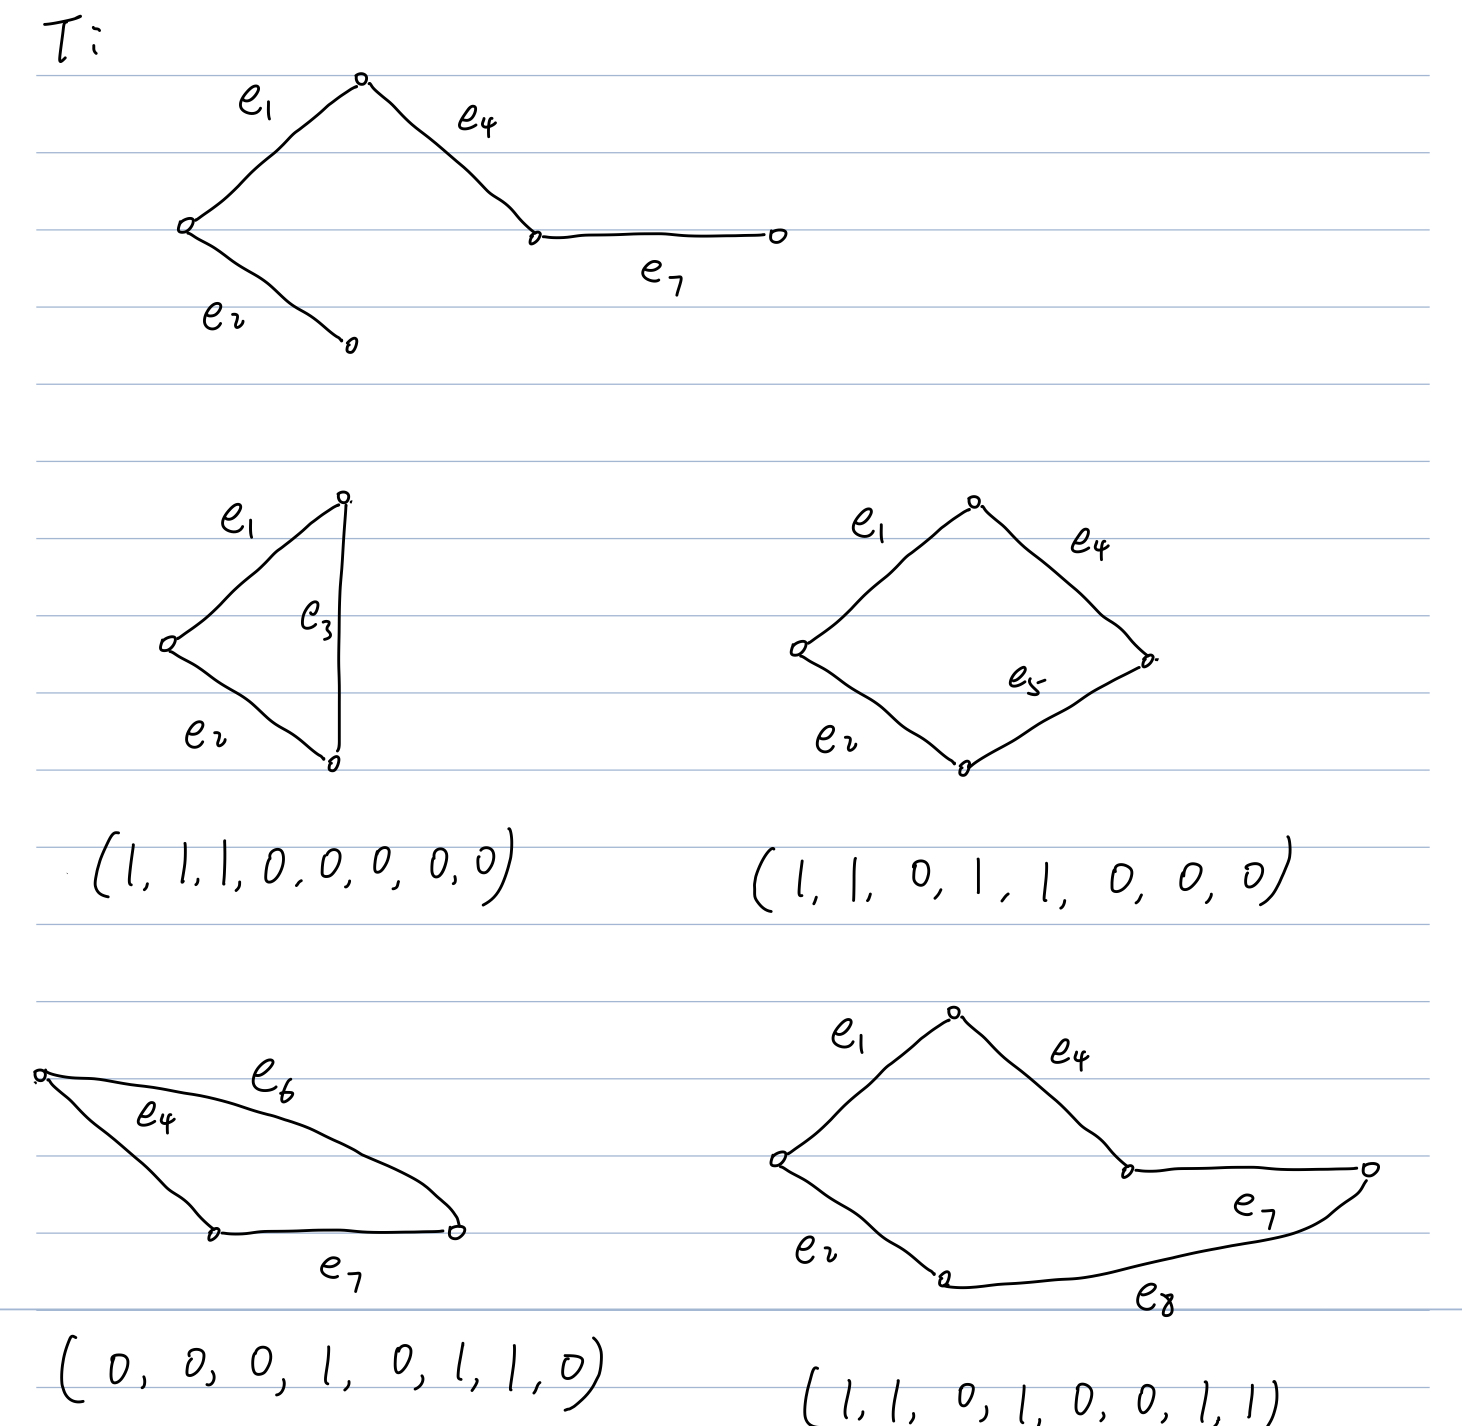
\includegraphics[scale=0.2]{1.PNG}
\end{figure*}

圈空间向量如图
\begin{figure*}[htbp]
    \centering
    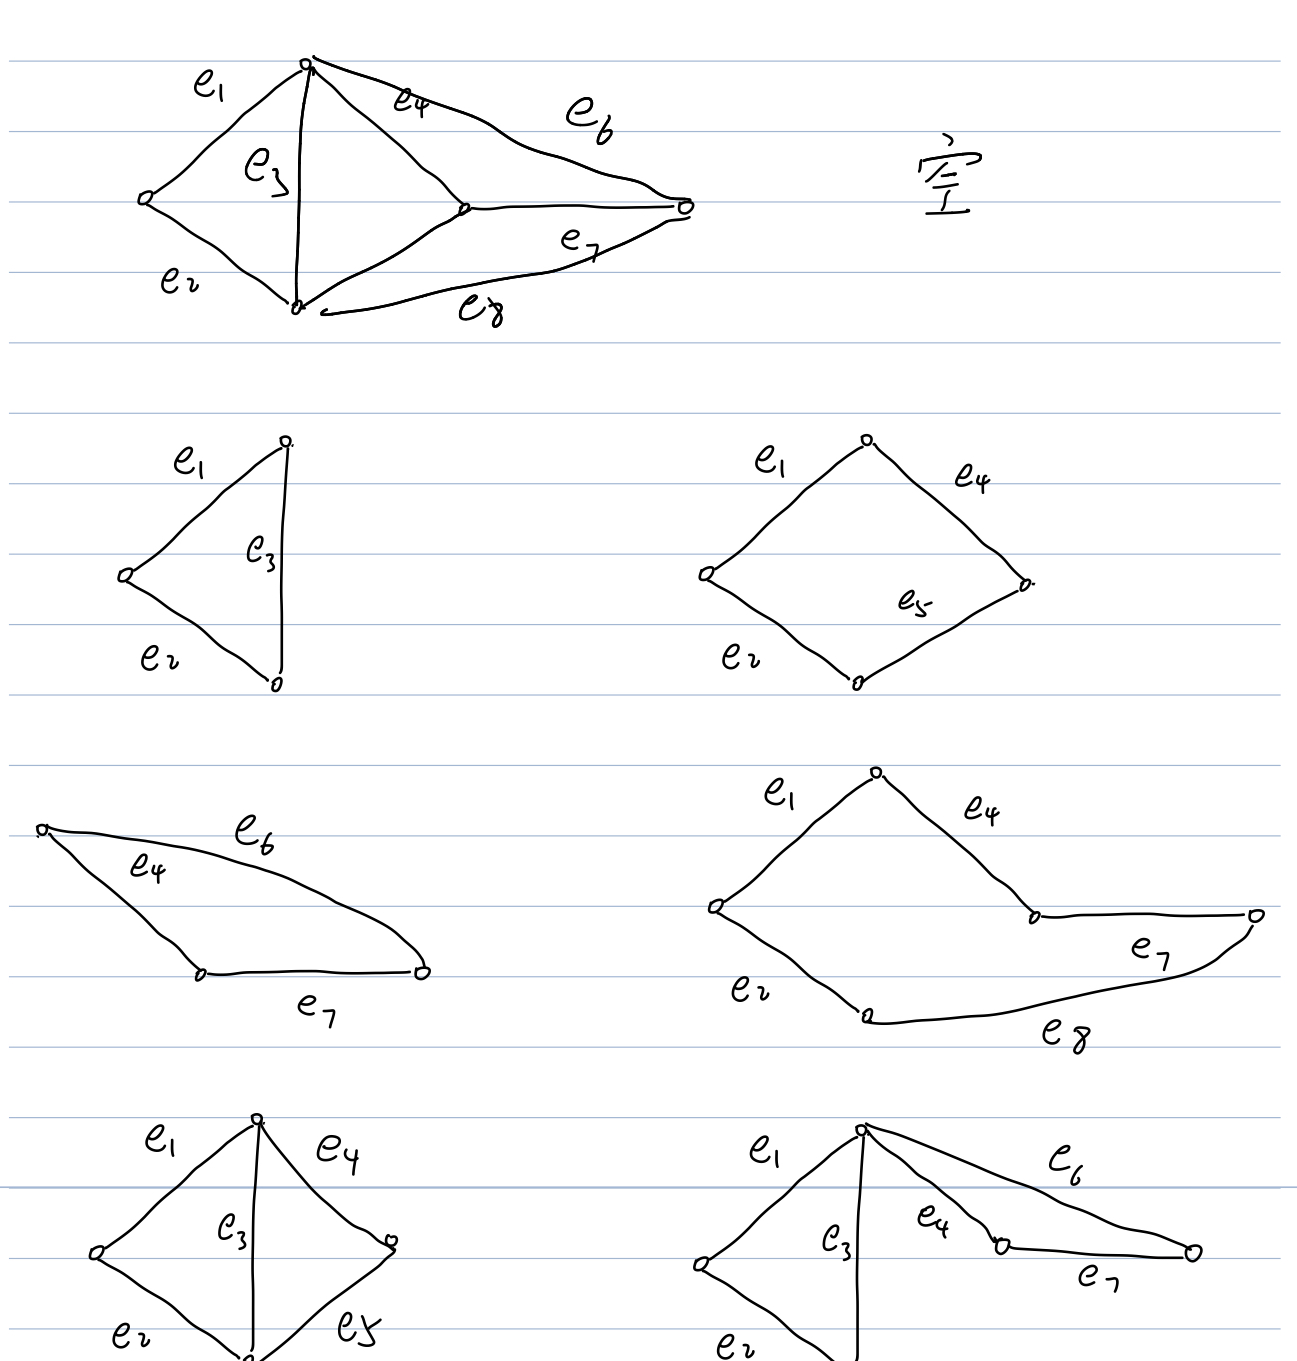
\includegraphics[scale=0.2]{2.PNG}
\end{figure*}

\begin{figure*}[htbp]
    \centering
    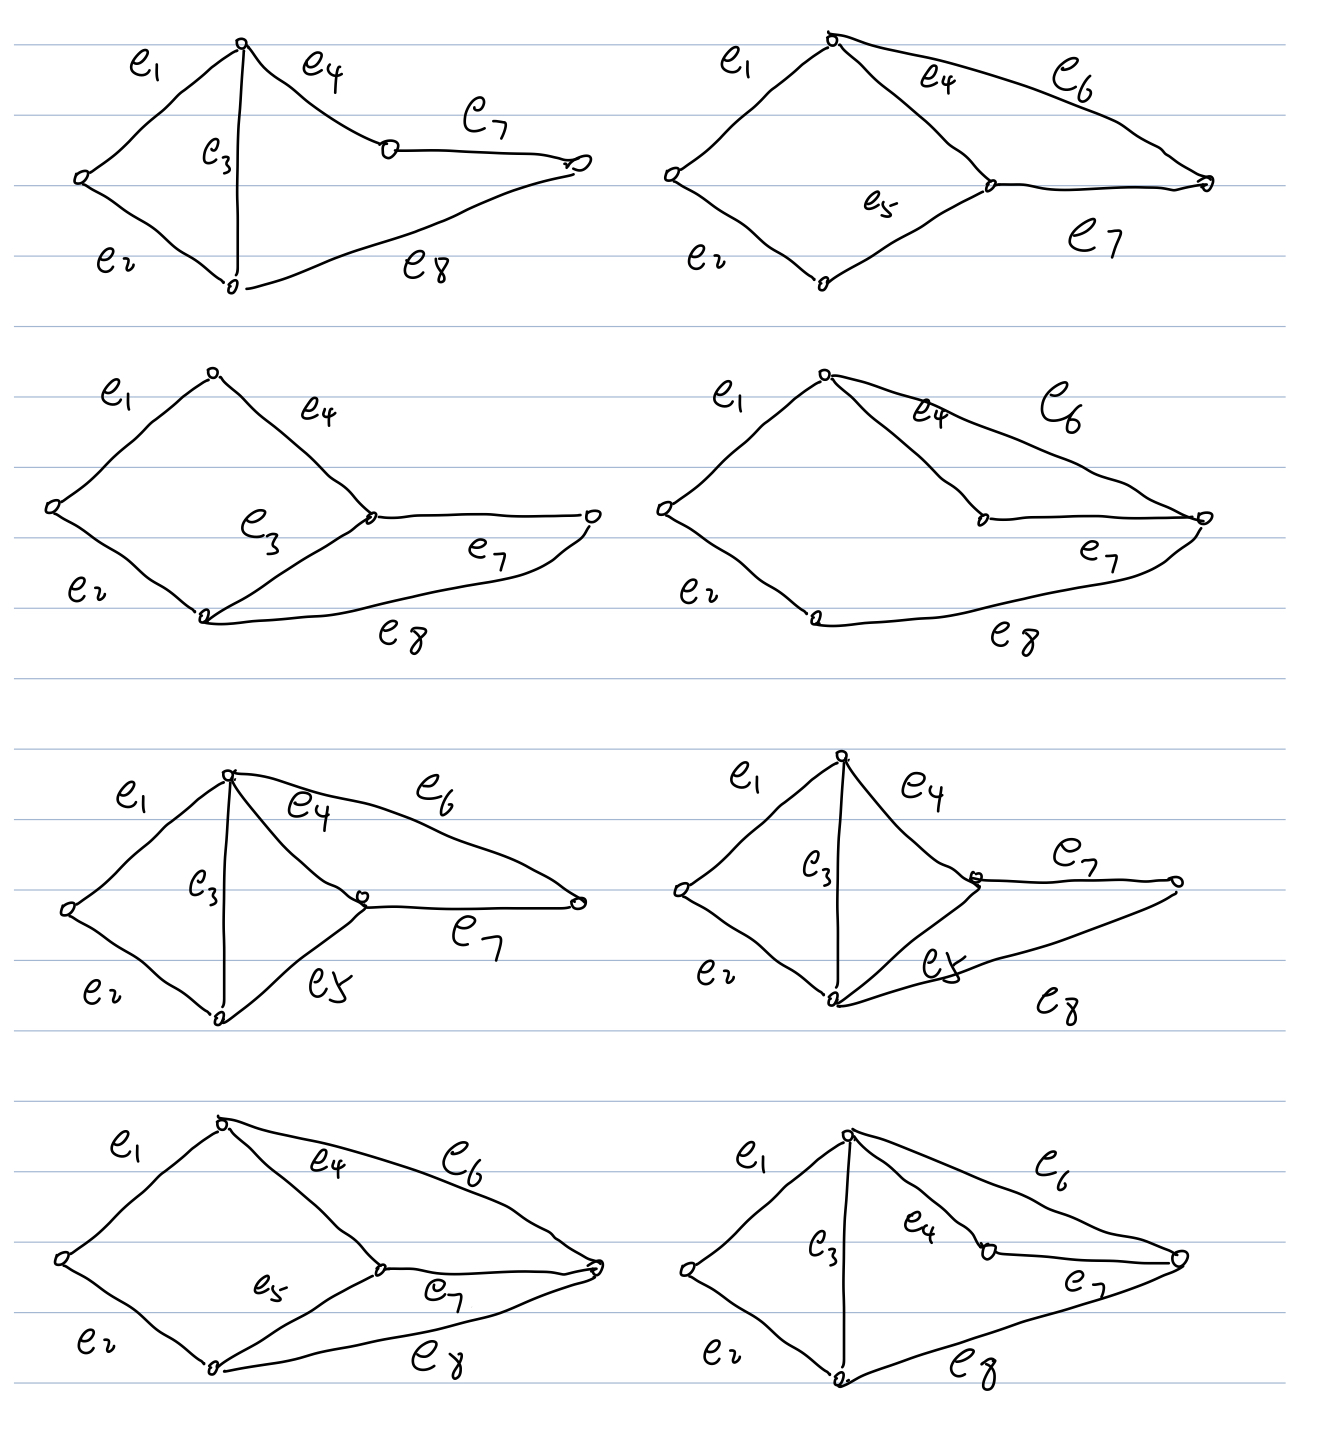
\includegraphics[scale=0.2]{3.PNG}
\end{figure*}


\subsection*{3.}
\begin{proof}
    我们将$G$中的边按照如下的方式编号:先将$S_1,S_2,\ldots,S_{\nu -1}$中在$T$上的那条边分别标记为$e_1,e_2,\ldots,e_{\nu -1}$,然后再将不在$T$上的边
    任意编号,前$\nu -1$个元素表示$T$的边,后$\varepsilon - \nu +1$个元素表示非$T$的边,则有:
    \[
        S_1= (1,0,\ldots,0,*,\ldots,*)
    \]
    \[
        S_2= (0,1,0,\ldots,0,*,\ldots,*)
    \]
    \[
        \ldots
    \]
    \[
        S_{\nu -1}= (0,\ldots,0,1,*,\ldots,*)
    \]
    给定一组常数$k_1,k_2,\ldots,k_{\nu -1}$,若$k_1 S_1+\ldots+k_{\nu -1} S_{\nu-1}$
\end{proof}

\end{document}